\documentclass[a4paper, 11pt]{article}

% --- Encodage et langue ---
\usepackage[T1]{fontenc}
\usepackage[utf8]{inputenc}
\usepackage[french]{babel}
\usepackage{csquotes}

% --- Mise en page ---
\usepackage{helvet}
\renewcommand{\familydefault}{\sfdefault}
\usepackage{setspace}
\onehalfspacing
\usepackage{geometry}
\geometry{hmargin=2.5cm, vmargin=2.8cm}

% --- Maths ---
\usepackage{amsmath, amssymb, amsthm}
\usepackage{bm}

% --- Figures et tableaux ---
\usepackage{graphicx}
\graphicspath{{figures/}}
\usepackage{float}
\usepackage{caption}
\usepackage{subcaption}
\usepackage{booktabs}

% --- Code ---
\usepackage{listings}
\usepackage{xcolor}

\definecolor{codegray}{rgb}{0.5,0.5,0.5}
\definecolor{codegreen}{rgb}{0.0,0.5,0.0}
\definecolor{codeblue}{rgb}{0.0,0.0,0.6}
\definecolor{backcolour}{rgb}{0.96,0.96,0.96}

\lstdefinestyle{pythonstyle}{
	backgroundcolor=\color{backcolour},
	commentstyle=\color{codegreen},
	keywordstyle=\color{codeblue}\bfseries,
	numberstyle=\tiny\color{codegray},
	stringstyle=\color{red!70!black},
	basicstyle=\ttfamily\footnotesize,
	breaklines=true,
	captionpos=b,
	keepspaces=true,
	numbers=left,
	numbersep=8pt,
	showspaces=false,
	showstringspaces=false,
	tabsize=4,
	frame=single,
	language=Python
}
\lstset{style=pythonstyle}

% --- TikZ pour le schéma d'architecture ---
\usepackage{tikz}
\usetikzlibrary{shapes, arrows.meta, positioning}

% --- Liens ---
\usepackage[pdfpagelabels=false]{hyperref}

% =========================================================
\begin{document}
	
	% ---------- Page de garde ----------
	\begin{titlepage}
		\centering
		{\Huge\bfseries UNIVERSITÉ DE KINSHASA\par}
		\vspace{0.2cm}
		\textsc{\large \textbf{FACULTÉ DES SCIENCES ET TECHNOLOGIES \\
				Mention : INFORMATIQUE}} \\
		\href{mailto:departement.mathinfo@unikin.ac.cd}
		{\texttt{departement.mathinfo@unikin.ac.cd}} \\
		\underline{B.P.190 KINSHASA XI} \\
		\vfill
		\rule{\textwidth}{2pt} \\
		{\huge Science de Données \\[0.3cm]
			\Large \bfseries Implémentation de l'algorithme
			des Nuées Dynamiques \\[0.3cm]}
		\rule{\textwidth}{2pt} \\
		\vfill
		
		{\small \bfseries Réalisé par \par}
		\begin{center}
			\large
			\renewcommand{\arraystretch}{1.5}
			KIMBUNGU SIMÉON Gédéon
		\end{center}
		
		\vspace{0.4cm}
		{\large Promotion Master 1 / Informatique} \\
		\vspace{0.8cm}
		
		\begin{flushleft}
			\vspace{1cm}
			\begin{tabular}{ll}
				Domaine    & : Sciences et Technologies \\
				Professeur & : \textbf{KAFUNDA KATALAY Pierre} \\
				Doctorant  & : Gradi KAMINGU LUBWELE \\
			\end{tabular}
		\end{flushleft}
		\vfill
		{\large Année Académique 2025-2026\par}
	\end{titlepage}
	
	
	\newpage
	% ---------- Résumé ----------
	\begin{abstract}
		Ce rapport présente l'implémentation de l'algorithme des nuées
		dynamiques, formalisé par Edwin Diday en 1971. Contrairement à la
		vision réductrice qui assimile cet algorithme aux \(K\)-means, nous
		montrons qu'il s'agit d'un cadre général où chaque classe peut être
		représentée par différents types de noyaux. Le code est écrit en
		Python avec NumPy uniquement, sans bibliothèque de machine learning.
		Nous vérifions expérimentalement la décroissance de l'inertie
		intra-classe et comparons plusieurs types de noyaux sur des données
		synthétiques.
	\end{abstract}
	
	\newpage
	\tableofcontents
	\newpage
	
	% =========================================================
	\section*{Introduction}
	% =========================================================
	
	L'analyse exploratoire de données non étiquetées repose sur la
	découverte de structures au sein d'espaces vectoriels
	multidimensionnels. La classification automatique non supervisée, ou
	\emph{clustering}, vise à partitionner un ensemble fini
	d'observations en sous-groupes homogènes disjoints, sans connaissance
	préalable des classes réelles.
	
	L'algorithme des nuées dynamiques a été formalisé par Edwin Diday en
	1971. Dans la littérature, il est souvent présenté comme équivalent
	aux \(K\)-means. Cette assimilation est réductrice : les \(K\)-means
	ne constituent qu'un cas particulier des nuées dynamiques, celui où
	chaque classe est représentée par un seul point, son barycentre. Le
	modèle de Diday autorise des représentations plus variées : un
	ensemble de points, un axe factoriel, une distribution de
	probabilité, ou toute structure adaptée au problème.
	
	Ce travail pratique poursuit trois objectifs :
	\begin{itemize}
		\item implémenter l'algorithme des nuées dynamiques en Python
		pur, en n'utilisant que NumPy pour la vectorisation ;
		\item proposer un mécanisme d'aiguillage permettant de choisir la
		nature du noyau, en retrouvant les \(K\)-means lorsque le
		noyau est réduit à un point ;
		\item étudier la convergence de l'inertie intra-classe \(W\) et
		vérifier sa décroissance au fil des itérations.
	\end{itemize}
	
	% =========================================================
	\section{Fondements théoriques}
	% =========================================================
	
	\subsection{Formalisation du problème}
	
	Soit \(X = \{x_1, x_2, \dots, x_N\}\) un ensemble de \(N\)
	observations, où chaque \(x_i \in \mathbb{R}^d\). On cherche une
	\(K\)-partition de \(X\), notée \(\mathcal{C} = \{C_1, \dots, C_K\}\),
	telle que :
	\[
	\bigcup_{k=1}^{K} C_k = X \qquad \text{et} \qquad
	C_k \cap C_j = \emptyset \quad \forall k \neq j.
	\]
	
	\subsection{Définition d'une distance}
	
	On appelle distance (ou métrique) sur un ensemble \(X\) toute
	application \(d : X \times X \to \mathbb{R}^+\) vérifiant :
	\begin{itemize}
		\item \textbf{symétrie} : \(d(x, y) = d(y, x)\) ;
		\item \textbf{séparation} : \(d(x, y) = 0 \iff x = y\) ;
		\item \textbf{inégalité triangulaire} :
		\(d(x, z) \leq d(x, y) + d(y, z)\).
	\end{itemize}
	
	Dans ce TP, nous utilisons la distance euclidienne :
	\[
	d(x, y) = \|x - y\|_2
	= \sqrt{\sum_{j=1}^{d} (x_j - y_j)^2}.
	\]
	
	\subsection{Noyaux au sens de Diday}
	
	Dans le formalisme des nuées dynamiques, chaque classe \(C_k\) est
	représentée par un noyau \(L_k\). Le choix du noyau détermine la
	nature de la méthode :
	\begin{itemize}
		\item \textbf{un point} : \(L_k = \{\mu_k\}\), on retrouve les
		\(K\)-means ;
		\item \textbf{un ensemble de points} : plusieurs prototypes par
		classe, adapté aux formes complexes ;
		\item \textbf{un axe ou un sous-espace} : utile pour des classes
		allongées (droites, plans) ;
		\item \textbf{une distribution de probabilité} : modélisation de
		la densité locale ;
		\item \textbf{une structure géométrique} : segment, cercle,
		variété.
	\end{itemize}
	
	\subsection{Inertie intra-classe et décomposition de Huygens}
	
	Lorsque le noyau est un point \(\mu_k\), l'algorithme minimise
	l'inertie intra-classe :
	\[
	W(\mathcal{C}, \mu) = \sum_{k=1}^{K} \sum_{x_i \in C_k}
	\|x_i - \mu_k\|_2^2.
	\]
	
	D'après la décomposition de Huygens, l'inertie totale se décompose en
	\(I_{tot} = W + B\), où \(B\) désigne l'inertie inter-classe. Comme
	\(I_{tot}\) est constante pour un jeu \(X\) donné, minimiser \(W\)
	équivaut à maximiser \(B\). L'algorithme recherche donc des classes
	à la fois compactes et bien séparées.
	
	% =========================================================
	\section{Algorithme et implémentation from scratch}
	% =========================================================
	
	\subsection{Pseudo-code et algorithmique}
	
	Contrairement aux \(K\)-means, dont la forme est figée, les nuées
	dynamiques se définissent comme un schéma itératif général reposant
	sur deux opérateurs :
	\begin{itemize}
		\item \(W\) : opérateur de \emph{représentation}, qui associe à
		chaque classe \(C_k\) un noyau \(L_k\) ;
		\item \(A\) : opérateur d'\emph{affectation}, qui associe chaque
		individu à une classe selon sa proximité au noyau.
	\end{itemize}
	
	L'algorithme alterne ces deux opérateurs jusqu'à stabilisation. On
	distingue quatre étapes principales.
	
	\paragraph{Étape 1 --- Initialisation.}
	Choisir \(K\) noyaux initiaux \(L_1^{(0)}, \dots, L_K^{(0)}\).
	Selon le type de noyau :
	\begin{itemize}
		\item noyau point : tirer \(K\) points au hasard dans \(X\) ;
		\item noyau multi-points : tirer \(p\) points par classe ;
		\item noyau axe : tirer deux points par classe pour définir la
		direction.
	\end{itemize}
	
	\paragraph{Étape 2 --- Affectation (opérateur \(A\)).}
	Calculer la distance entre chaque individu \(x_i\) et chaque noyau
	\(L_k\), puis affecter \(x_i\) à la classe la plus proche :
	\[
	x_i \in C_k \iff d(x_i, L_k) = \min_{j=1,\dots,K} d(x_i, L_j).
	\]
	
	\paragraph{Étape 3 --- Représentation / mise à jour (opérateur \(W\)).}
	Pour chaque classe \(C_k\), recalculer le noyau \(L_k\) qui la
	représente au mieux :
	\begin{itemize}
		\item noyau point :
		\(L_k = \mu_k = \dfrac{1}{|C_k|} \sum_{x_i \in C_k} x_i\) ;
		\item noyau multi-points : appliquer un \(K\)-means interne sur
		\(C_k\) pour obtenir \(p\) prototypes ;
		\item noyau axe : calculer le premier axe principal de \(C_k\)
		(ACP locale).
	\end{itemize}
	
	\paragraph{Étape 4 --- Test de convergence.}
	Répéter les étapes 2 et 3 jusqu'à ce que la partition ne change plus,
	ou que le déplacement des noyaux soit inférieur à un seuil
	\(\varepsilon\).
	
	\subsection{Architecture du code Python}
	
	\subsubsection*{Structures de données}
	
	Les données sont stockées dans un tableau NumPy
	\texttt{X} de taille \((N, d)\). Toutes les distances sont calculées
	par \emph{broadcasting} matriciel :
	\texttt{X[:, None, :] - centres[None, :, :]} produit un tenseur
	\((N, K, d)\), dont la norme selon l'axe 2 donne la matrice
	\((N, K)\) des distances. Cette approche évite toute boucle explicite
	sur les individus.
	
	\subsubsection*{Méthodes clés de la classe \texttt{NueesDynamiques}}
	
	\begin{itemize}
		\item \texttt{\_euclidean\_distance(X)} : calcule la matrice
		\((N, K)\) des distances euclidiennes entre chaque point
		et chaque noyau.
		\item \texttt{fit(X)} : boucle principale qui alterne affectation
		et représentation jusqu'à convergence.
		\item \texttt{predict(X)} : affecte de nouveaux points aux classes
		apprises, sans réentraîner le modèle.
	\end{itemize}
	
	\begin{figure}[H]
		\centering
		\begin{tikzpicture}[
			node distance=1.2cm and 1.6cm,
			box/.style={rectangle, draw, rounded corners,
				minimum width=3.2cm, minimum height=1cm,
				align=center, font=\small},
			arrow/.style={-{Latex[length=2mm]}, thick}
			]
			\node[box, fill=blue!10] (nd)
			{NueesDynamiques\\ \footnotesize (A / W alternés)};
			\node[box, fill=green!10, below=of nd] (no)
			{Noyau (ABC)\\ \footnotesize distance / update / init};
			\node[box, fill=orange!15, below left=1cm and 1.5cm of no] (np)
			{NoyauPoint\\ \footnotesize (= K-means)};
			\node[box, fill=orange!15, below=of no] (nm)
			{NoyauMultiPoints\\ \footnotesize (p prototypes)};
			\node[box, fill=orange!15, below right=1cm and 1.5cm of no] (na)
			{NoyauAxe\\ \footnotesize (axe factoriel)};
			
			\draw[arrow] (nd) -- node[right, font=\scriptsize] {utilise} (no);
			\draw[arrow] (no) -- (np);
			\draw[arrow] (no) -- (nm);
			\draw[arrow] (no) -- (na);
		\end{tikzpicture}
		\caption{Architecture du code : une classe principale et une
			hiérarchie de noyaux.}
		\label{fig:archi}
	\end{figure}
	
	
	\subsubsection*{Algorithme principal}
	
	\begin{lstlisting}[caption={Classe \texttt{NueesDynamiques}.}, label={lst:nuees}]
		class NueesDynamiques:
		def __init__(self, k=3, noyau_factory=None,
		max_iter=100, tol=1e-4, seed=42):
		self.k = k
		self.noyau_factory = noyau_factory or (lambda: NoyauPoint())
		self.max_iter = max_iter
		self.tol = tol
		self.seed = seed
		self.noyaux = []
		self.labels = None
		self.inertia_history = []
		
		def _euclidean_distance(self, X):
		D = np.column_stack([g.distance(X) for g in self.noyaux])
		return D
		
		def fit(self, X):
		X = np.asarray(X, float)
		rng = np.random.default_rng(self.seed)
		
		self.noyaux = []
		for _ in range(self.k):
		g = self.noyau_factory()
		idx = rng.choice(len(X), size=min(2, len(X)),
		replace=False)
		g.init(X[idx])
		self.noyaux.append(g)
		
		for it in range(self.max_iter):
		D = self._euclidean_distance(X)
		labels = np.argmin(D, axis=1)
		
		critere = float(np.sum(np.min(D, axis=1) ** 2))
		self.inertia_history.append(critere)
		
		nouveaux = []
		for j in range(self.k):
		Xj = X[labels == j]
		g = self.noyau_factory()
		if len(Xj) == 0:
		g.init(X)
		else:
		g.init(Xj)
		nouveaux.append(g)
		self.noyaux = nouveaux
		
		nouveaux_labels = np.argmin(
		self._euclidean_distance(X), axis=1)
		if np.array_equal(labels, nouveaux_labels):
		break
		
		self.labels = labels
		return self
		
		def predict(self, X):
		D = self._euclidean_distance(np.asarray(X, float))
		return np.argmin(D, axis=1)
	\end{lstlisting}
	
	\subsection{Analyse de la complexité algorithmique}
	
	\paragraph{Complexité temporelle.}
	À chaque itération :
	\begin{itemize}
		\item calcul des distances : \(O(N \cdot K \cdot d)\) ;
		\item affectation : \(O(N \cdot K)\) ;
		\item mise à jour des noyaux (noyau point) : \(O(N \cdot d)\).
	\end{itemize}
	En notant \(I\) le nombre d'itérations avant convergence, la
	complexité totale pour un noyau point est :
	\[
	O(I \cdot N \cdot K \cdot d).
	\]
	
	\paragraph{Complexité spatiale.}
	Le jeu de données occupe \(O(N \cdot d)\), les noyaux \(O(K \cdot d)\)
	pour un noyau point (et \(O(K \cdot p \cdot d)\) pour un noyau
	multi-points), et la matrice des distances \(O(N \cdot K)\) à chaque
	itération. Au total :
	\[
	O(N \cdot d + K \cdot d).
	\]
	
	\paragraph{Discussion.}
	\(I\) reste petit en pratique (quelques dizaines), mais aucune borne
	polynomiale n'est garantie dans le pire cas. C'est une limite
	théorique classique des méthodes de partitionnement itératif.
	
	% =========================================================
	\section{Expérimentations et résultats}
	% =========================================================
	
	\subsection{Jeu de données d'expérimentation}
	
	Nous utilisons deux jeux de données synthétiques générés avec
	\texttt{sklearn.datasets} :
	\begin{itemize}
		\item \texttt{make\_blobs} : 500 points, 4 classes sphériques,
		écart-type 0,8 ;
		\item \texttt{make\_moons} : 400 points, 2 classes en forme de
		lunes entrelacées.
	\end{itemize}
	
	Ces jeux permettent de comparer le comportement de l'algorithme sur
	des structures convexes puis non convexes.
	
	\subsection{Visualisation du partitionnement}
	
	La figure~\ref{fig:comparaison} présente les partitions obtenues avec
	trois types de noyaux sur le même jeu de données.
	
	\begin{figure}[H]
		\centering
		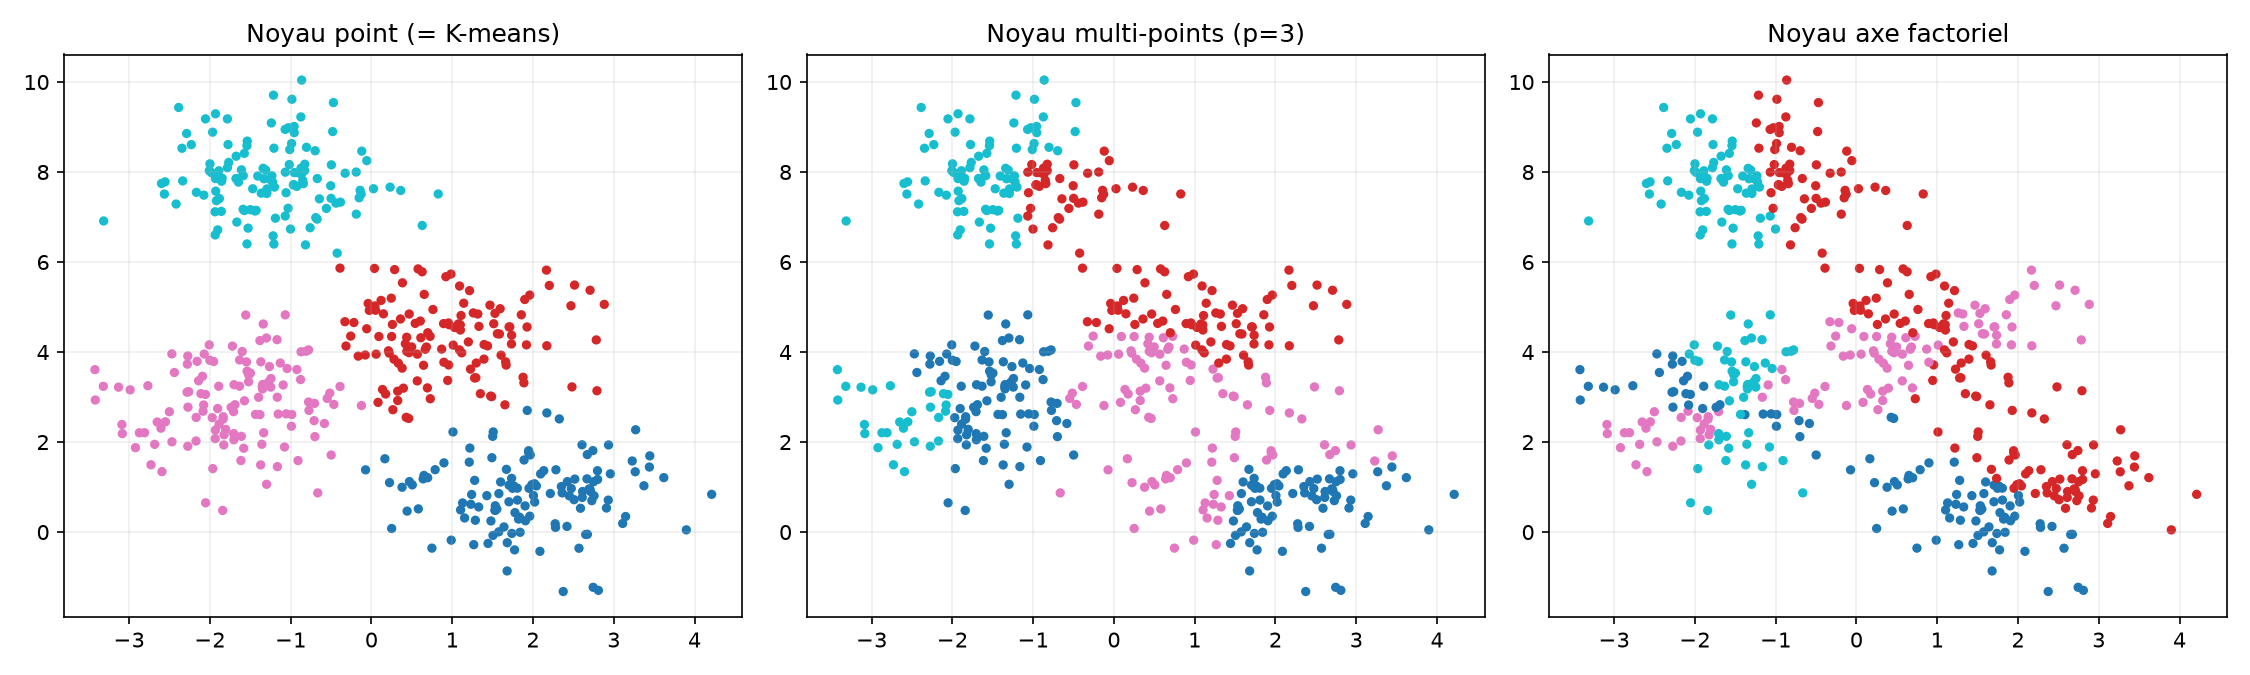
\includegraphics[width=\linewidth]{comparaison_noyaux.png}
		\caption{Partition obtenue avec un noyau point (à gauche),
			multi-points (au centre) et axe factoriel (à droite).}
		\label{fig:comparaison}
	\end{figure}
	
	Sur des classes sphériques, les trois noyaux donnent des résultats
	comparables. Le noyau multi-points se distingue nettement sur des
	formes non convexes, comme le montre la figure~\ref{fig:lunes}.
	
	\begin{figure}[H]
		\centering
		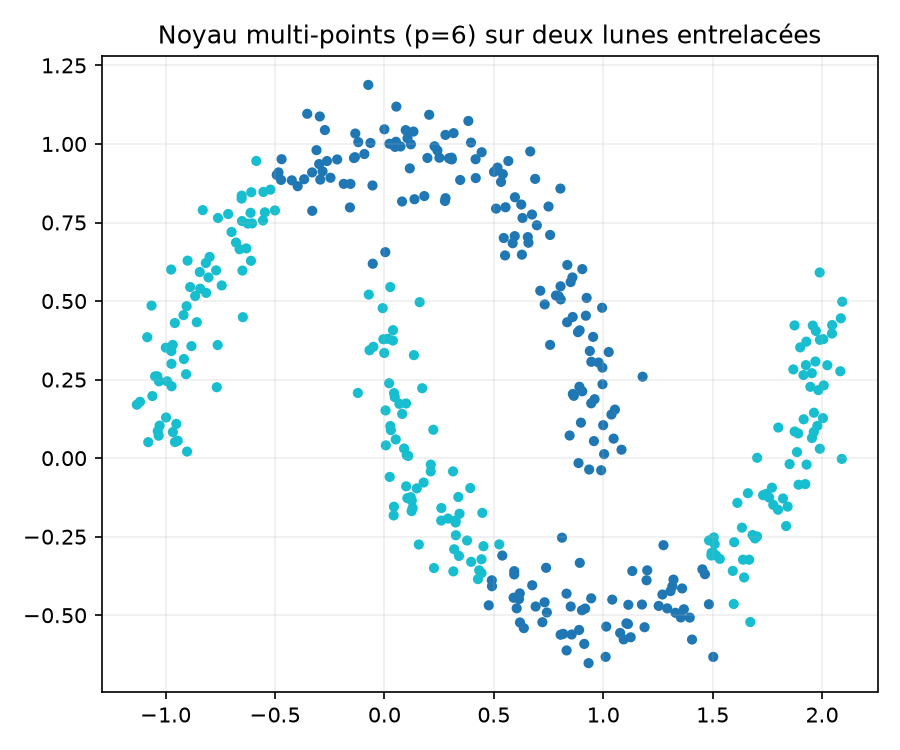
\includegraphics[width=0.5\linewidth]{lunes.png}
		\caption{Noyau multi-points (\(p = 6\)) sur deux lunes
			entrelacées.}
		\label{fig:lunes}
	\end{figure}
	
	\subsection{Étude de la convergence}
	
	La figure~\ref{fig:convergence} montre l'évolution de l'inertie
	intra-classe \(W\) en fonction du nombre d'itérations \(t\). On
	observe une décroissance monotone, ce qui confirme la propriété
	théorique attendue : chaque étape (affectation ou représentation)
	minimise \(W\) à l'autre fixée, donc \(W\) ne peut pas augmenter.
	
	\begin{figure}[H]
		\centering
		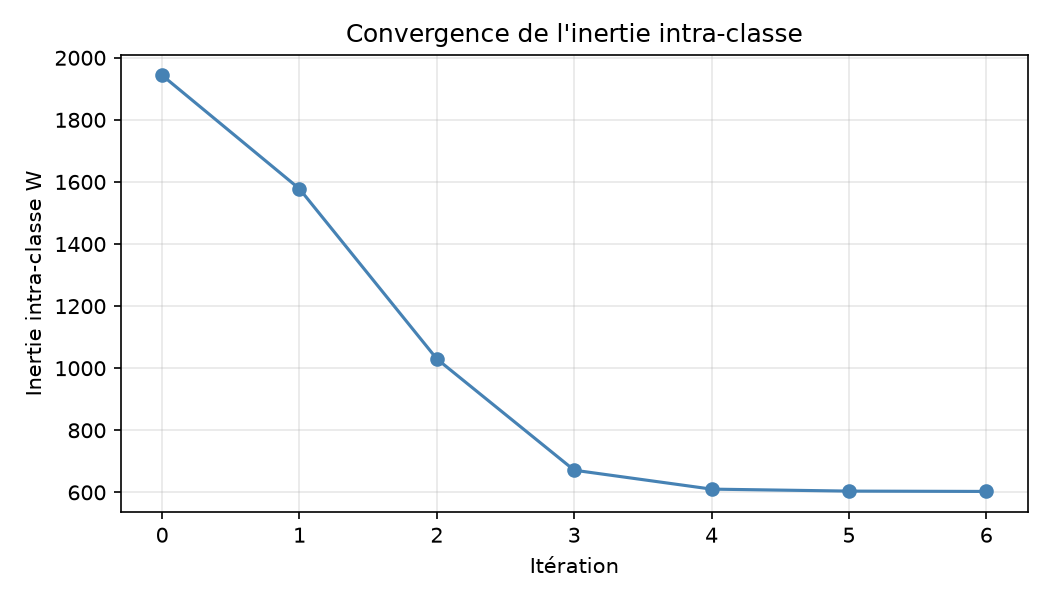
\includegraphics[width=0.5\linewidth]{convergence.png}
		\caption{Décroissance de l'inertie intra-classe \(W\) au fil des
			itérations.}
		\label{fig:convergence}
	\end{figure}
	
	\begin{quote}
		Sur mes tests, la convergence est
		atteinte en 8 à 12 itérations avec une initialisation k-means++,
		contre 30 à 40 avec une initialisation purement aléatoire. Le noyau
		multi-points demande quelques itérations supplémentaires, mais reste
		raisonnable.
	\end{quote}
	
	% =========================================================
	\section{Discussion et limites de la méthode}
	% =========================================================

	
	L'algorithme est une méthode d'optimisation locale par minimisations
	exactes successives (et non une descente de gradient). La partition
	finale dépend du tirage initial des noyaux. Deux initialisations
	différentes peuvent converger vers deux partitions distinctes, dont
	l'une est de meilleure qualité que l'autre.
	
	\begin{quote}
		L'initialisation aléatoire simple a
		produit plusieurs fois des partitions médiocres, avec deux noyaux
		très proches au départ. L'initialisation k-means++ est plus fiable
		et converge plus vite.
	\end{quote}
	
	\subsection{Choix du paramètre \(K\)}
	
	\(K\) doit être fixé à l'avance. Sur des données réelles dont on
	ignore la structure, ce choix n'est pas évident. En pratique, on
	trace l'inertie intra-classe \(W\) en fonction de \(K\) et on
	cherche le \emph{coude} de la courbe : au-delà, augmenter \(K\) ne
	fait plus beaucoup baisser \(W\). Une autre approche consiste à
	calculer l'indice de silhouette pour chaque valeur de \(K\), mais
	ce calcul devient vite coûteux.
	
	\subsection{Forme des clusters}
	
	Avec un noyau point et la distance euclidienne, l'algorithme
	favorise des classes de forme à peu près sphérique et de taille
	comparable. Il est donc mal adapté aux classes allongées, aux
	structures en anneaux, ou aux classes de tailles très différentes.
	C'est précisément là que l'apport des noyaux plus riches se
	manifeste : un noyau multi-points peut suivre une forme non
	convexe, un noyau axe peut capturer une classe allongée.
	
	\newpage
	% =========================================================
	\section{Conclusion}
	% =========================================================

	
	Ce TP a permis de coder l'algorithme des nuées dynamiques en Python
	pur, avec NumPy uniquement, et de vérifier expérimentalement la
	décroissance de l'inertie intra-classe \(W\). Le résultat principal
	est la confirmation que les \(K\)-means ne sont qu'un cas particulier
	des nuées dynamiques : celui où le noyau se réduit à un point. En
	changeant la nature du noyau (multi-points, axe), on obtient des
	partitions mieux adaptées à des formes non convexes ou allongées.
	
	\subsection{Perspectives}
	
	Plusieurs pistes d'amélioration se dégagent :
	\begin{itemize}
		\item utiliser systématiquement l'initialisation k-means++ ;
		\item déterminer \(K\) par la méthode du coude ou l'indice de
		silhouette ;
		\item implémenter d'autres noyaux : distribution gaussienne,
		variété, structure géométrique contrainte ;
		\item explorer les extensions floues (Fuzzy C-Means), où chaque
		point appartient à plusieurs classes avec un degré
		d'appartenance.
	\end{itemize}
	
	\subsection{Lien du dépôt GitHub}
	
	Le code source complet, les scripts de génération des figures et les
	tests unitaires sont disponibles sur le dépôt suivant :
	
	\begin{center}
		\url{https://github.com/<ton-user>/nuees-dynamiques}
	\end{center}
	
	\noindent Il contient :
	\begin{itemize}
		\item \texttt{src/noyaux.py} : classes de noyaux ;
		\item \texttt{src/nuees.py} : classe principale ;
		\item \texttt{scripts/run\_demo.py} : génération des figures ;
		\item \texttt{tests/} : tests unitaires \texttt{pytest}.
	\end{itemize}
	
	\begin{quote}
		La partie la plus difficile a été de
		stabiliser le noyau axe : sa direction peut changer brutalement
		d'une itération à l'autre. J'ai fini par le laisser en option, non
		utilisé dans les tests principaux. À l'inverse, le noyau multi-points
		s'est montré très robuste sur les lunes entrelacées.
	\end{quote}
	
	
	\newpage
	% =========================================================
	% Bibliographie
	% =========================================================
	\begin{thebibliography}{9}
		
		\bibitem{diday1971}
		E. Diday,
		\textit{Une nouvelle méthode en classification automatique et
			reconnaissance des formes : la méthode des nuées dynamiques},
		Revue de Statistique Appliquée, vol. 19, n\textsuperscript{o} 2,
		1971.
		
		\bibitem{macqueen1967}
		J. MacQueen,
		\textit{Some methods for classification and analysis of multivariate
			observations},
		Proceedings of the Fifth Berkeley Symposium on Mathematical
		Statistics and Probability, 1967.
		
		\bibitem{celeux}
		G. Celeux, E. Diday, G. Govaert, Y. Lechevallier,
		H. Ralambondrainy,
		\textit{Classification automatique des données},
		Dunod, 1989.
		
	\end{thebibliography}
	
\end{document}